\documentclass[12pt,a4paper]{article}

% Single-column research paper template adapted from the provided
% IGI Global book chapter template. Citations and references use APA style.

\usepackage[a4paper,margin=1in]{geometry}
\usepackage{setspace}
\usepackage{amsmath,amssymb,amsfonts}
\usepackage{graphicx}
\usepackage{array}
\usepackage{multirow}
\usepackage{caption}
\usepackage{float}
\usepackage{placeins}
\usepackage{url}
\usepackage{iftex}
\usepackage[american]{babel}
\usepackage{csquotes}

\ifXeTeX
\usepackage{fontspec}
\setmainfont{Times New Roman}
\setsansfont{Times New Roman}
\setmonofont{Times New Roman}
\else
\usepackage{mathptmx}
\fi

% Compile with Biber so APA-style citations and references are generated correctly.
\usepackage[style=apa,backend=biber,sorting=nyt,sortcites=true]{biblatex}
\usepackage[hidelinks]{hyperref}

\addbibresource{references.bib}

\onehalfspacing
\setlength{\parindent}{0.5in}
\setlength{\parskip}{0pt}
\setcounter{secnumdepth}{0}
\captionsetup{font=normalsize,labelfont=bf,labelsep=period}
\emergencystretch=3em
\Urlmuskip=0mu plus 1mu\relax

\makeatletter
\renewcommand{\@maketitle}{%
  \newpage
  \null
  \vskip 2em%
  \begin{center}%
    {\fontsize{14}{16.8}\selectfont\bfseries \@title \par}%
    \vskip 1.5em%
    {\fontsize{12}{14.4}\selectfont
      \lineskip .5em%
      \begin{tabular}[t]{c}%
        \@author
      \end{tabular}\par}%
    \vskip 1em%
    {\fontsize{12}{14.4}\selectfont \@date}%
  \end{center}%
  \par
  \vskip 1.5em}
\renewcommand{\section}{\@startsection{section}{1}{0pt}%
  {1.5\baselineskip}{0.75\baselineskip}%
  {\normalfont\fontsize{13}{15.6}\selectfont\bfseries}}
\renewcommand{\subsection}{\@startsection{subsection}{2}{0pt}%
  {1.25\baselineskip}{0.5\baselineskip}%
  {\normalfont\fontsize{13}{15.6}\selectfont\bfseries}}
\renewcommand{\subsubsection}{\@startsection{subsubsection}{3}{0pt}%
  {1\baselineskip}{0.25\baselineskip}%
  {\normalfont\fontsize{13}{15.6}\selectfont\itshape}}
\makeatother

\title{Enhancing Network Brute Force Attack Detection: A Hybrid Sampling and Ensemble Learning Approach}

\author{
\fontsize{12}{14.4}\selectfont
Edward Aria Tanujaya\\
Computer Science Department, School of Computer Science\\
Bina Nusantara University, Jakarta, Indonesia 11480\\
edward.tanujaya001@binus.ac.id\\
0009-0001-2374-7153
\and
\fontsize{12}{14.4}\selectfont
Andrian Pratama\\
Computer Science Department, School of Computer Science\\
Bina Nusantara University, Jakarta, Indonesia 11480\\
andrian.pratama@binus.ac.id\\
0009-0009-1573-7068
\and
\fontsize{12}{14.4}\selectfont
Jeta Sunanda\\
Computer Science Department, School of Computer Science\\
Bina Nusantara University, Jakarta, Indonesia 11480\\
jeta.sunanda@binus.ac.id\\
0009-0003-7942-1667 
\and
\fontsize{12}{14.4}\selectfont
Hidayaturrahman\\
Computer Science Department, School of Computer Science\\
Bina Nusantara University, Jakarta, Indonesia 11480\\
hidayaturrahman@binus.ac.id\\
0000-0001-5005-8006
\and
\fontsize{12}{14.4}\selectfont
Satriadi Putra Santika\\
Computer Science Department, School of Computer Science\\
Bina Nusantara University, Jakarta, Indonesia 11480\\
satriadi.santika@binus.ac.id\\
0009-0006-0937-473X
}

\date{}

\begin{document}
\sloppy

\maketitle

\section{Abstract}
Machine-learning-based Network Intrusion Detection Systems (NIDS) are widely used to detect malicious traffic, but their performance can decline when attack classes are severely underrepresented. Previous studies have attempted to mitigate this problem through feature selection, sampling, and ensemble learning. However, these components often fail to adequately address minority attacks. In datasets such as CICIDS2017, Brute Force traffic remains difficult to detect because repeated authentication attempts can resemble benign activity. This study evaluates a Brute-Force-centered CICIDS2017 pipeline that integrates train-only feature selection, SMOTE-Tomek hybrid sampling, and ensemble learning. The workflow consolidates CICIDS2017 labels into eight classes, limits the dominant Benign class, removes invalid records, selects numerical flow features using ANOVA \textit{SelectKBest} and correlation pruning, and applies resampling only to the training partition. Validation results showed that SMOTE-Tomek achieved the strongest macro F1-score among the sampling strategies, while the Stacking Ensemble achieved the best macro F1-score among classifier candidates. SMOTE-Tomek increased Brute Force training representation from 5,204 to 76,385 samples and reduced the imbalance against DDoS from about 30.30:1 to 2.06:1. On the unseen test set, the selected configuration achieved 99.93\% macro accuracy, 86.10\% macro precision, 90.22\% macro recall, 86.93\% macro F1-score, and 97.98\% macro ROC-AUC. For Brute Force traffic, it achieved 98.70\% precision, 92.66\% recall, 95.58\% F1-score, and 0.0253\% FPR. The findings indicate that SMOTE-Tomek and heterogeneous stacking can improve Brute Force detection under multiclass imbalance.

\section{Keywords}
Network Intrusion Detection System, Brute Force Detection, CICIDS2017, SMOTE-Tomek, Ensemble Learning

\section{INTRODUCTION}

Internet-based communication is now central to file sharing, remote access, and daily computing, but the same connectivity also expands the attack surface for private and organizational data. Recent threat reports show that cyberattacks continue to grow in both volume and stealth: malware-free detections increased from 62\% in 2021 to 71\% in 2022, while 75\% of attacks used to gain initial access were malware-free in 2023.\footnote{CrowdStrike Global Threat Reports, 2023 and 2024.} This trend shows that network defense requires detection mechanisms that can recognize suspicious behavior beyond known malware signatures.

Intrusion Detection Systems (IDS) are security mechanisms that monitor system or network activity and generate alerts when malicious behavior is detected \parencite{singh2022minority}. IDS can be categorized into Host-based IDS (HIDS) and Network-based IDS (NIDS). HIDS monitors host-level information such as logs and resource usage, while NIDS observes network traffic flows. In this study, NIDS is selected because network-flow monitoring is suitable for detecting attack behavior across communication traffic and can be managed more centrally than host-by-host monitoring \parencite{almuhanna2025anomaly,irfaissurur2025web}. Flow-based detection is also practical for machine learning because a bidirectional communication session can be represented by numerical attributes such as packet length, duration, timing, port, and flag information. These attributes do not describe user intent directly, but they provide measurable traces of behavior that can be learned by classifiers.

As network data continues to grow, traditional IDS approaches face difficulty in recognizing new or changing attack behavior. Machine learning and deep learning have therefore been used to improve NIDS because they can learn patterns from traffic data rather than relying only on fixed signatures \parencite{almuhanna2025anomaly,ahmed2024explainable}. However, ML-based NIDS still has important weaknesses, including high false-positive rates, difficulty generalizing to imbalanced data, high computational cost from redundant features, and deployment challenges in real-time environments \parencite{almuhanna2025anomaly,alsaffar2024shielding,alessa2024hybrid,yang2024imbalanced,prasad2025optimizing}. These weaknesses are especially important when the target class is rare. A classifier can appear accurate by learning the dominant normal or high-volume attack classes, while still failing to detect attack types that appear in much smaller quantities.

Previous studies have attempted to reduce these weaknesses through feature selection, sampling, and ensemble learning. Feature selection can remove redundant network-flow attributes, hybrid sampling can reduce class imbalance, and ensemble learning can combine diverse classifiers to improve robustness. However, these components are often evaluated separately or without sufficient focus on minority attacks. CICIDS2017 is a common NIDS benchmark that includes Brute Force traffic, but its class distribution is highly imbalanced, which makes minority-attack detection difficult \parencite{harini2023minority,irfaissurur2025web,khan2024balanced,le2024unbalanced}. This is important because Brute Force attacks do not always appear as high-volume traffic. Brute force attacks work by sending login or authentication requests that generate flow patterns similar to legitimate access or benign data. Therefore, the model needs to distinguish between timing, service access, packet behavior, and protocol-state indicators.

Hybrid sampling methods such as SMOTE-Tomek address class imbalance by oversampling minority classes and cleaning majority or boundary samples \parencite{khan2024balanced,le2024unbalanced,nassreddine2025ensemble}. SMOTE generates synthetic minority samples, while Tomek-link cleaning removes samples located near overlapping class boundaries. However, Brute Force traffic remains difficult to detect because repeated authentication attempts may resemble legitimate user behavior, which can lead to false alarms or missed detections when only one classifier is used \parencite{rihan2023iot,irfaissurur2025web}. For this reason, sampling needs to be supported by feature selection and an appropriate classifier design. The model should use a reduced feature set to limit redundant attributes and combine classifiers that can capture different patterns in multiclass traffic.

This study evaluates the performance of a multiclass Network Intrusion Detection System in detecting Brute Force attacks. The proposed approach combines selected flow features, SMOTE-Tomek applied only to the training data, and ensemble learning. The data are split first to prevent data leakage. Then, feature selection and resampling are then applied only during to the training data, while the validation and test data remain in their original form. Surely, the final results can be evaluated more reliably on unseen test data.

The main contributions of this study are as follows: (1) developing an integrated CICIDS2017 pipeline that combines label consolidation, Benign-class limitation, train-only feature selection, and SMOTE-Tomek resampling; (2) comparing sampling methods and classifier models for Brute Force detection using validation results; (3) evaluating the selected Stacking Ensemble with SMOTE-Tomek using macro-level and Brute-Force-specific metrics; and (4) interpreting the selected flow features in relation to Brute Force behavior. Together, these contributions show how each part of the pipeline supports the detection of the target attack class, not only the final model performance.

\section{LITERATURE REVIEW}

Machine-learning-based IDS models are commonly used to analyze network traffic with high-dimensional features and imbalanced attack classes. Many studies address these problems through feature selection, resampling, or ensemble classifiers, although these strategies are often evaluated separately. However, these components are closely related: feature selection affects which traffic patterns are learned, resampling influences how minority attacks appear during training, and ensemble methods can reduce classification errors from individual models. This indicates a research gap in evaluating whether the combined use of these strategies can improve minority-class detection, particularly for Brute Force attacks that are often underrepresented in intrusion detection datasets.

\subsection{Feature Selection and Dimensionality Reduction in NIDS}

Feature selection plays an important role in NIDS because redundant flow-based attributes can increase training cost and weaken model generalization \parencite{nassreddine2025ensemble,alsaffar2024shielding,khan2024balanced,selvakumar2025feature,yu2025attack}. Network-flow datasets often contain related measurements, such as duration, packet counts, byte counts, timing values, and flag indicators. If all features are used without screening, the model may learn repeated information, require higher computation, and become more sensitive to noise. Therefore, feature selection is useful not only for reducing dimensionality, but also for identifying traffic behaviors that are most relevant for intrusion detection.

Several previous studies have shown the benefit of feature selection in NIDS. \textcite{nassreddine2025ensemble} combined correlation-based selection with embedded XGBoost feature selection and retained 10 features before applying KNN-DT-RF-XGBoost stacking, achieving 99.97\% accuracy and 99.93\% F1-score on CIC-IDS2017. \textcite{alsaffar2024shielding} used MI-Boruta with RF-XGBoost-CatBoost-MLP stacking and reported 99.92\% multiclass accuracy on CICIDS2017. Meanwhile, \textcite{khan2024balanced} applied SelectKBest, correlation reduction, and SMOTE-Tomek with conventional classifiers, where Decision Tree and AdaBoost reached 96.37\% accuracy and 96.33\% F1-score in multiclass classification. These findings indicate that feature selection is an important early step before modeling high-dimensional traffic data.

In the context of Brute Force detection, feature selection should not be treated only as a routine preprocessing step. The selected attributes need to reflect patterns related to repeated service access, timing behavior, packet characteristics, and TCP-state differences, since Brute Force traffic can appear similar to normal login or access activity. For this reason, this study combines ANOVA-based univariate selection with correlation pruning. ANOVA is used to rank features based on their ability to distinguish class labels, while correlation pruning removes highly redundant attributes from the ranked feature set. This approach is simpler than wrapper-based methods and fits the controlled experimental design because it keeps the process interpretable while reducing the feature space before resampling and ensemble training.

\subsection{Handling Imbalanced Datasets Using Hybrid Sampling}

Hybrid sampling is often used to remove ambiguous or noisy samples to improve the visibility of minority-class samples during training \parencite{harini2023minority,prasad2025optimizing,yang2024imbalanced}. Imbalance is a persistent difficulty in intrusion detection because benign traffic and high-volume attack classes can dominate the training distribution. When this happens, a classifier can minimize overall error while still under-detecting rare but important attacks. For minority attacks, the problem is not only the small number of samples but also the limited diversity of attack patterns observed during training. Oversampling can make the minority class more visible, while cleaning methods help reduce overlap between minority and majority samples.

The combination of SMOTE with K-means undersampling and XGBoost classification was used by SKM-XGB to achieve 97.49\% multiclass detection on UNSW-NB15 and 99.22\% on NSL-KDD \parencite{hooshmand2024robust}. CICIDS2017 was balanced using SMOTE-Tomek to reach 96.37\% multiclass accuracy with Decision Tree and AdaBoost \parencite{khan2024balanced}. SMOTE-Tomek was also used prior to stacking to reach 99.97\% accuracy and 99.93\% F1 score on CIC-IDS2017 \parencite{nassreddine2025ensemble}. These studies suggest that SMOTE-Tomek is relevant for Brute Force attack detection because it combines synthetic minority generation with boundary cleaning. 

Sampling can create evaluation bias if it is applied before data splitting, because synthetic samples may indirectly influence the validation or test partitions. To avoid this risk, this study applies sampling only to the training data, while keeping the validation and test sets in their original class distribution. This setting provides a more realistic evaluation of Brute Force detection, since the model must recognize Brute Force samples in an imbalanced traffic environment rather than in an artificially balanced test set.


\subsection{Ensemble Learning Approaches for Intrusion Detection}

Ensemble learning is useful in IDS because combining diverse classifiers can offset the limitations of individual models \parencite{emanet2023voting,pramanick2025stacking,wardana2024collaborative,gu2025semisupervised,alsubaei2025smart}. In network-flow data, different classifiers may capture different types of relationships: tree-based models handle nonlinear feature interactions, boosting models improve difficult decision boundaries, distance-based methods reflect local sample structure, and linear meta-learners provide a simple way to combine base-model outputs. This diversity is especially relevant in imbalanced NIDS, where minority attacks may not be captured well by a single decision rule.

\textcite{farooqi2024enhancing} proposed a voting ensemble using Decision Tree, Random Forest, and XGBoost, achieving 99.98\% accuracy on CIC-IDS2017 with a very low false positive rate. \textcite{urmi2024stacked} applied RF, XGBoost, and Extra Trees as base learners with Logistic Regression as the stacking model, reporting 99.90\% accuracy and 99.80\% F1-score on CICIDS2017. Meanwhile, \textcite{alessa2024hybrid} evaluated RF, XGBoost, and MLP through voting and stacking, with soft voting reaching 99.9\% accuracy and 99.8\% F1-score on InSDN. Based on these studies, this research uses Random Forest, Decision Tree, XGBoost, KNN, and Logistic Regression as baseline and ensemble components.

Voting and stacking are two common ensemble strategies. In soft voting, class probabilities from several models are averaged, which can make predictions more stable when the individual models are already reliable. Stacking trains a meta-learner to combine base-model outputs and can therefore learn which base learners are more useful for different decision regions. This study evaluates both strategies because Brute Force detection requires not only high overall correctness, but also balanced minority-class behavior. The comparison helps determine whether probability averaging or meta-learning is more suitable after SMOTE-Tomek resampling.

\subsection{Research Gap}

Many of current studies have done techniques such as feature selection, sampling, or ensemble learning, but only few report how to enhance the minority attack, such as brute force in a multiclass. This Network Intrusion Detection System (NIDS) challenge is still be remaining challenge on many experiments \parencite{xu2025fewshot,wardana2024collaborative}. A model may perform well on multiclass metrics, but still lost on a specific minority attack such as brute force. On detecting brute force attack, it is required specific class interpretation because the cost of missed attacks and false alarms is different from the cost of other classes.

This research is addressed that gap of the lower metrics on brute force attacks by combining the techniques such as ANOVA feature selection, correlation pruning, SMOTE-Tomek , and two ensemble strategies such as soft voting and stacking. This research also makes the comparasion between sampling techniques such as no sampling, SMOTE, Tomek-Links, and SMOTE-Tomek, in order to validate which one is the best technique for addressing the imbalance dataset. 

Even though many IDS studies report the high accuracy, but they don't interpret it well when one or two classes dominate the dataset. For Brute Force attacks detection, the more useful evidence is shows whether the model can maintain precision, recall, and F1-score. This research treats the accuracy just as a part of evaluation, and gives more attention on macro F1-score. This shift focus is necessary because the intended is to improve detection on a specific minority classes attack rather than on overall multiclass.

\section{METHODOLOGY/DATA AND METHODS}

This section describes the workflow used to evaluate Brute Force detection in a multiclass NIDS. As shown in Figure~\ref{fig:method_pipeline}, the experiment begins with CICIDS2017 label mapping and Benign-class limitation, followed by data cleaning, numerical feature retention, stratified splitting, train-only feature selection, train-only SMOTE-Tomek resampling, ensemble model development, validation diagnostics, and final test evaluation. The workflow was designed to answer a practical modeling problem: whether Brute Force detection can be improved without allowing validation or test data to influence feature selection or resampling.

All leakage-sensitive steps were fitted only on the training partition, while validation and test data remained unresampled. This design is important because oversampling before splitting can create synthetic samples that are too closely related to validation or test records. Similarly, feature selection fitted on the full dataset can transfer information from the evaluation data into the training process. By fitting feature selection and sampling only within the training workflow, the experiment preserves a clearer separation between model development and final evaluation.

\begin{figure}[H]
\centering
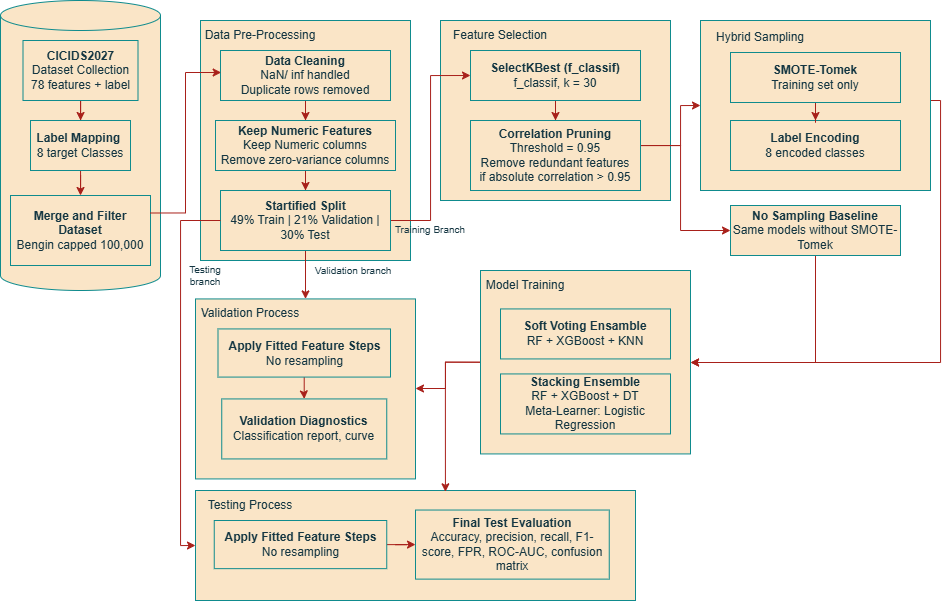
\includegraphics[width=0.95\linewidth]{Flowchart}
\caption{Overall research workflow from dataset preparation to final evaluation.}
\label{fig:method_pipeline}
\caption*{\textit{Source:} Authors' processing, 2026.}
\end{figure}

\subsection{Dataset}

CICIDS2017 is a public benchmark from the Canadian Institute for Cybersecurity, University of New Brunswick, containing 2,830,743 labeled bidirectional flow records with 78 features and one label \parencite{khan2024balanced,nassreddine2025ensemble}. The raw labels were consolidated into eight categories: \texttt{BENIGN} to Benign; \texttt{Bot} to Bot; DoS labels, \texttt{DDoS}, and \texttt{Heartbleed} to DDoS; \texttt{PortScan} to Port Scan; \texttt{Infiltration} to Infiltrations; Patator and Web Attack-Brute Force labels to Brute Force; XSS labels to XSS; and \texttt{Sql Injection} to SQL-Injection. No labels were dropped after mapping. To reduce normal-traffic dominance while retaining attack samples, Benign was randomly limited to 100,000 records using random seed 42. The resulting class counts are shown in Table~\ref{tab:class_dist}.

The label consolidation step was used to make the classification task more suitable for Brute-Force-centered multiclass evaluation. Several original CICIDS2017 labels represent related attack behavior, and grouping them into broader categories reduces unnecessary fragmentation while preserving the main attack families. Brute Force was formed from Patator and Web Attack-Brute Force labels because both represent repeated authentication or access attempts. The Benign limitation was applied to reduce the dominance of normal traffic, but attack classes were retained after mapping so that the minority-class structure of the dataset remained visible.

\begin{table}[H]
\caption{Class Distribution Across Main Processing Stages}
\label{tab:class_dist}
\centering
\scriptsize
\renewcommand{\arraystretch}{1.15}
\setlength{\tabcolsep}{3pt}
\resizebox{\linewidth}{!}{%
\begin{tabular}{|l|r|r|r|}
\hline
\textbf{Label} & \textbf{Cleaned} & \textbf{Train Before} & \textbf{Train After} \\
\hline
Benign & 97,947 & 47,994 & 76,724 \\
\hline
Bot & 1,953 & 957 & 76,996 \\
\hline
Brute Force & 10,622 & 5,204 & 76,385 \\
\hline
DDoS & 321,775 & 157,669 & 157,551 \\
\hline
Infiltrations & 36 & 17 & 77,000 \\
\hline
Port Scan & 90,819 & 44,501 & 76,842 \\
\hline
SQL-Injection & 21 & 11 & 76,999 \\
\hline
XSS & 652 & 320 & 76,400 \\
\hline
\end{tabular}
}
\caption*{\textit{Note.} Train After refers to the training partition after SMOTE-Tomek resampling.}
\end{table}

Table~\ref{tab:class_dist} shows that the dataset remained strongly imbalanced even after Benign limitation. DDoS remained the largest attack category with 321,775 cleaned records, while Brute Force contained 10,622 cleaned records. Other attack classes were much smaller, including 652 XSS records, 36 Infiltrations records, and 21 SQL-Injection records. This distribution confirms that the experiment was not only a general multiclass classification task, but also a minority-attack detection task. It also justifies the use of macro metrics, because overall accuracy would be dominated by larger classes if each class were not considered separately.

\subsection{Data Preprocessing}

Data preprocessing was performed to improve data quality and model reliability on CICIDS2017. The cleaning stage removed invalid records, redundant entries, and missing values so that the classifiers were not trained on incomplete or duplicated observations. The numerical attributes is kept because the selected model require numerical input, and also because CICIDS2017 features are primarily represented as quantitative network measurements.

To preserve the original class proportions during evaluation, stratified splitting was used for the train-validation-test partitions. The initial split allocated 70\% of the data to training, 30\% to testing. The training data was then split using the stratified k-fold method into four folds for training data and one fold for validation data. This was done to allow cross-validation during the training and validation processes. Stratification was also maintained during five-fold validation so that each fold contained a proportional representation of the available classes. This was necessary because some attack categories, especially SQL-Injection and Infiltrations, contained very few samples after preprocessing. Without stratification, a fold could contain too few minority samples to provide meaningful validation feedback.

The test data was completely kept hidden from the model selection process. Sampling techniques selection, classifier selection, and feature selection were only done for training and validation. The test data was only used after everything was finished to see how the model performs on data that it has never seen before. This way can make sure that the result was reliable and trusted, also the model really works in the real world scenario.

\subsection{Feature Selection}

\textit{SelectKBest} with \texttt{f\_classif} was implemented to improve interpretability and reduce dimensionality. To prevent data leakage, the selector was used only for the training set, this step is crucial for ensuring the validation and test data remained unseen during ranking the feature. top 30 features was selected by \textit{SelectKBest} with \texttt{f\_classif}, the reason is because it ranks numerical attributes based on their ability to separate discrete class labels. 

After ranking the feature, correlation pruning was used to the selected feature. The redudant features were removed if their absolute correlation coefficient more than the constraints \(|r| > 0.95\). The process reduced the input space from 70 numerical features to 16 final features. This reduction allowed the ensemble models to focus on a smaller group of discriminative and less redundant variables.

Feature selection was performed before resampling so that synthetic samples were generated in the reduced feature space. This sequence prevents synthetic data from influencing which features are selected. It also reduces the computational burden of SMOTE-Tomek because the sampler operates on fewer dimensions.

\subsection{Imbalanced Data Handling}

To determine the sampling method, this research evaluated four strategies: no sampling, SMOTE, Tomek Links, and SMOTE-Tomek. A Decision Tree classifier was used during this sampling-selection stage so that the sampling methods could be compared under the same classifier setting. No sampling served as the baseline, SMOTE represented oversampling, Tomek Links represented boundary cleaning, and SMOTE-Tomek represented a hybrid approach.

The selection was based on macro validation metrics because the target problem is imbalanced. Macro metrics give each class equal weight, so they are more informative than accuracy when minority attacks are important. SMOTE increases the number of minority samples by creating synthetic examples, but synthetic samples may appear near regions where minority and majority classes overlap. Tomek Links can remove ambiguous boundary samples, but cleaning alone does not increase minority-class exposure. SMOTE-Tomek was therefore selected because it combines the strengths of both approaches: it increases minority representation and removes overlapping or ambiguous samples after oversampling.

In this experiment, SMOTE-Tomek was applied only to the training data. The validation and test partitions were not resampled, because the goal was to evaluate the model on data distributions that were not artificially balanced. This design is especially relevant for Brute Force traffic, because operational NIDS data are expected to remain imbalanced even if the training procedure uses resampling.

\subsection{Proposed Ensemble Models}

After the sampling method was selected, two ensemble models were developed: a soft voting ensemble and a stacking ensemble. The soft voting model combined Random Forest, XGBoost, and KNN by averaging their predicted class probabilities, with \texttt{n\_jobs}=1. This strategy was used to obtain a more stable prediction by combining probability outputs from different base learners. The stacking ensemble used Random Forest, XGBoost, and Decision Tree as base learners, while Logistic Regression was used as the meta-learner. It was trained using five-fold internal cross-validation with \texttt{n\_jobs}=1. Unlike soft voting, stacking does not simply average predictions, but learns how to combine the outputs of the base models through the meta-learner.

The Random Forest model used 300 trees, a maximum depth of 20, balanced class weights, random seed 42, and \texttt{n\_jobs}=-1. XGBoost was configured with 300 estimators, maximum depth 8, learning rate 0.05, subsample 0.8, column subsample 0.8, histogram tree method, \texttt{device=cuda}, \texttt{mlogloss}, and random seed 42. The Decision Tree model used a maximum depth of 20, balanced class weights, and random seed 42. Logistic Regression was configured with \(C=0.5\), 2000 maximum iterations, balanced class weights, random seed 42, and \texttt{n\_jobs}=-1. KNN used \(k=3\), Euclidean distance, and \texttt{n\_jobs}=-1. These models were selected because previous NIDS studies have shown strong performance from tree-based models, boosting methods, KNN, voting ensembles, and stacking ensembles for imbalanced intrusion detection \parencite{farooqi2024enhancing,urmi2024stacked,nassreddine2025ensemble}.

The selected model set was intentionally heterogeneous. Random Forest and Decision Tree provide tree-based decision structures, XGBoost adds boosted tree learning, KNN introduces a local distance-based perspective, and Logistic Regression serves as a simple meta-learning layer for stacking. This diversity is useful because Brute Force traffic may be distinguished from benign traffic using different types of evidence, such as service ports, timing patterns, and packet-level characteristics.


\subsection{Experimental Setup}

The experiment was run in Google Colab with an NVIDIA L4 GPU. The python notebook needs to install several required libraries like \texttt{imbalanced-learn}, \texttt{xgboost} \(\geq\) 2.0.0, \texttt{seaborn}, and \texttt{joblib}. But, the version of these packages were not written. Random seeds of 42 was in the way to make the process more easy to repeat, more likely for when splitting the data, initiate the model and sampling process. However, this setup may leads to different results, because the factors like different computer or use newer version of google colab and package.

The workflow included of two selection process and followed by the final testing. First, the sampling techniques were compared using validation metrics, with a Decision Tree as classifier model. Second, classifier performance was evaluated after the selected sampling method had been fixed. The last configuration, is combined the Stacking and Soft Voting Ensembles with SMOTE-Tomek, were trained using the both training and validation data, then tested on the hidden test set or unseen set. This design ensure that the final model not only chosen based on unseen set or test set results, thereby this design also maintaining the integrity of the evaluation and providing a realistic estimate systems.

\subsection{Evaluation Metrics}

This study used metrics evaluation like accuracy, precision, recall, F1-score, false positive rate (FRP), and macro F1-Score. This metric was chosen because it provide overall model performance. Accuracy shows overall proportion of correct prediction, but this study doesn't use it as the main metric, the reason is the CICIDS2017 dataset is remained imbalanced after limiting the Benign class. Therefore, the model can still obtain high accuracy on majority classes, but the ability to detect minority classes may remain weak. 

Because of this issue, this study more emphasis on metrics such as precision, recall, F1-Score, and FPR, especially for the Brute Force class. Precision showed how the model really predicted Brute Force attack, so, this can test the reliability of the model. Recall showed how many times was the model correct on detecting the brute force samples. F1-score shows the balance between precision and recall. FPR showed how many times was the model incorrectly on detecting the brute force samples. These metrics are important, because it can keep the false alarms at a low level and the intrusion detection system model can still detect the attacks.

Macro-averaged metrics were also applied to evaluate the model fairly on all of classes. Since every class receives same weight in macro averaging, the result makes minority classes was seen more, because the large classess such as DDoS and Benign was less dominated. This result shows the relevancy with this study, because the main objective is not only gain high overall classification perfomance, but also to check, test, and assess whether the model can handle the minority classes. 'One Vs Rest' method was used to calculate the results for each specific attack. For example. if one attack was picked up such as Brute Force, it is called as positive group, and the other will be called as negative group. This do one by one for each class. The terms \(\mathrm{TP}\), \(\mathrm{TN}\), \(\mathrm{FP}\), and \(\mathrm{FN}\) denote true positives, true negatives, false positives, and false negatives, respectively. The metrics were calculated as follows:

\noindent\textbf{1. Accuracy:} Accuracy represents the ratio of correctly classified samples to the total number of evaluated samples.
\begin{equation}
\mathrm{Accuracy} = \frac{\mathrm{TP}+\mathrm{TN}}{\mathrm{TP}+\mathrm{TN}+\mathrm{FP}+\mathrm{FN}}
\label{eq:accuracy}
\end{equation}

\noindent\textbf{2. Precision:} Precision shows the proportion of positive predictions that were correctly classified.
\begin{equation}
\mathrm{Precision} = \frac{\mathrm{TP}}{\mathrm{TP}+\mathrm{FP}}
\label{eq:precision}
\end{equation}

\noindent\textbf{3. Recall:} Recall indicates the proportion of actual positive samples that were correctly detected by the model.
\begin{equation}
\mathrm{Recall} = \frac{\mathrm{TP}}{\mathrm{TP}+\mathrm{FN}}
\label{eq:recall}
\end{equation}

\noindent\textbf{4. F1-score:} F1-score combines precision and recall using the harmonic mean, making it useful when both missed detections and false alarms need to be considered.
\begin{equation}
\mathrm{F1} = \frac{2 \times \mathrm{Precision} \times \mathrm{Recall}}{\mathrm{Precision}+\mathrm{Recall}}
\label{eq:f1}
\end{equation}

\noindent\textbf{5. False Positive Rate:} FPR measures the proportion of negative samples that were incorrectly predicted as positive.
\begin{equation}
\mathrm{FPR} = \frac{\mathrm{FP}}{\mathrm{FP}+\mathrm{TN}}
\label{eq:fpr}
\end{equation}

Because of the high accuracy may leads to overfitting, like high accuracy may hide weak detection on the minority attack. This study gives more attention on Brute Force precision, recall, F1-score, and FPR. These metrics will provide the clear indication of whether the porposed model can detect Brute Force trafic effectively without producing excessive false alarms.

During the sampling and classifier selection stages, the same metric was also used. Marco metrics were used to determine which one the best sampling method that can improved the imbalanced classes of CICIDS2017 dataset perfomance rather than only for increasing the total number of correct predictions in the sampling selection. Also, macro F1-score was used in the classifier selection, because it shows the balance between precision and recall while every class is denoted as equally importance. The test evaluation reports both macro level metrics and Brute Force specific metrics, so the selected model can be analyzed from overall multiclass robustness, and target attack detection performance.

\FloatBarrier

\section{RESULTS AND DISCUSSION}

This section discusses the main results obtained from the experiment, focusing on the effect of class balancing, the selected flow features, and the performance of each classifier. Since the dataset was still imbalanced, the discussion does not rely only on accuracy. A high accuracy score can still be misleading when the model performs well on dominant classes but fails to detect smaller attack classes.

For this reason, the interpretation gives more attention to macro F1-score, macro recall, macro FPR, and Brute-Force-specific results. These metrics are more useful for understanding whether the proposed pipeline actually improves Brute Force detection, rather than only increasing the overall number of correct predictions. The following discussion therefore connects the validation and test results with the main objective of this study, which is to improve Brute Force detection under multiclass imbalance.

\subsection{Effect of Hybrid Sampling on Class Representation}

Table~\ref{tab:sampling_selection_macro} shows the five-fold validation results used to select the sampling strategy. SMOTE-Tomek achieved the strongest macro F1-score at 83.83\%, the highest macro precision at 83.85\%, the highest macro recall at 89.10\%, and the highest macro ROC-AUC at 94.99\%. Tomek Links produced the highest macro accuracy at 99.93\% and the lowest macro FPR at 0.0450\%, but its macro F1-score was lower than the no-sampling baseline.

\begin{table}[H]
\caption{Sampling Method Selection Based on Validation Macro Performance}
\label{tab:sampling_selection_macro}
\centering
\scriptsize
\renewcommand{\arraystretch}{1.15}
\setlength{\tabcolsep}{3pt}
\resizebox{\linewidth}{!}{%
\begin{tabular}{|l|r|r|r|r|r|r|}
\hline
\textbf{Sampling Method} & \textbf{Macro Acc.} & \textbf{Macro Prec.} & \textbf{Macro Rec.} & \textbf{Macro F1} & \textbf{Macro FPR} & \textbf{Macro ROC-AUC} \\
\hline
No Sampling & 99.92\% & 80.05\% & 88.09\% & 82.02\% & 0.0484\% & 94.35\% \\
\hline
SMOTE & 99.91\% & 82.86\% & 88.41\% & 82.99\% & 0.0519\% & 94.60\% \\
\hline
SMOTE-Tomek & 99.91\% & 83.85\% & 89.10\% & 83.83\% & 0.0508\% & 94.99\% \\
\hline
Tomek & 99.93\% & 79.65\% & 86.43\% & 81.20\% & 0.0450\% & 93.42\% \\
\hline
\end{tabular}
}
\caption*{\textit{Note.} Sampling strategies were evaluated with a Decision Tree classifier across five validation folds.}
\end{table}

The meaning of this result is that cleaning majority-boundary samples alone can reduce false positives, but it does not necessarily improve class-balanced detection. SMOTE-Tomek was stronger because it combined synthetic minority oversampling with Tomek-link cleaning. In the final training partition, Brute Force increased from 5,204 to 76,385 samples after SMOTE-Tomek. Relative to DDoS, the largest attack class, the Brute Force imbalance changed from approximately 30.30:1 before resampling to 2.06:1 after resampling. This does not make the dataset perfectly uniform, because DDoS remained larger than the other classes, but it substantially reduced the pressure that previously made Brute Force easier to overlook during model fitting.

This finding is consistent with studies showing that hybrid sampling can improve minority-attack representation in imbalanced intrusion datasets \parencite{khan2024balanced,le2024unbalanced,nassreddine2025ensemble,harini2023minority}. The selection of SMOTE-Tomek is therefore justified because it improved the most important macro-balanced indicators while also increasing the Brute Force training representation substantially. The implication is that resampling should not be judged only by overall accuracy, because the accuracy differences among sampling methods were very small. Consequently, SMOTE-Tomek became the most appropriate sampling method for this pipeline because it gave Brute Force traffic a more meaningful role in model learning without discarding the multiclass structure of the dataset.

The comparison also shows why a hybrid method is preferable to using only one balancing mechanism. SMOTE improved macro F1-score compared with no sampling, but SMOTE-Tomek produced a further improvement while also achieving the strongest macro ROC-AUC among the sampling candidates. Tomek Links alone produced the lowest macro FPR, but its lower macro recall and macro F1-score indicate that cleaning without increasing minority exposure was not sufficient for the target problem. The consequence is that the sampling choice should be interpreted as a balance between representation and boundary control. For Brute Force detection, increasing representation is essential because the original training data contain far fewer Brute Force samples than DDoS samples.

The result also explains why the final discussion does not treat every minority class as equally improved. SMOTE-Tomek created a much larger training representation for rare classes, but the quality of synthetic expansion still depends on the information available in the original samples. Brute Force had enough original support to benefit from resampling more reliably than SQL-Injection or Infiltrations. Therefore, the sampling result supports the main objective of improving Brute Force detection, while also showing that extremely small classes require more cautious interpretation.

\subsection{Selected Flow Features and Detection Meaning}

The feature-selection process reduced the original numerical feature space to 16 final features through ANOVA-based \textit{SelectKBest} and correlation pruning. Permutation-importance diagnostics showed that Destination Port was the most influential feature. The remaining high-ranked features were grouped into four flow-behavior categories: TCP window behavior, timing behavior, packet behavior, and TCP flag behavior.

These features show patterns that make sense for catching Brute Force attacks. These features capture the critical network characteristics such as the TCP initial window behavior, arrival timing, connection duration, variation of size of the packet, traffic rate and TCP flag behavior. The specific habits earned from brute force attacks are they keep attacking the same service, repeatedly, and regularly, so the useful indicators are destination service information, timing, length of the packet, and TCP-state.

The result supports claim of previous NIDS studies to use feature selection in order to address the redudant flow attributes before classification \parencite{nassreddine2025ensemble,alsaffar2024shielding}. Also, supports the claim of the studies that treat Brute Force and web attacks as behavior-driven detection problems rather than just as volume-drive anomalies \parencite{rihan2023iot,irfaissurur2025web}. The selected features was used because they are not only statistically important, but also meaningful in terms of how Brute Force traffic appears in network flows. This also means that the model did not only guess based on hidden math, but also it used network data that actually make sense for human. As the consequent, the result also shows the pratical credibility of the pipeline for CICIDS 2017 Brute Force attack detection, but do the validation is still required for the same important patterns that appear in different datasets before make a claim that this model works well on everything.

This explanation is important because feature importance alone can lead to misleading if the selected features do not have clear behavioral connection with the target. In this study, chosen Destination Port as the most important feature, which can be make sense because Brute Force attacks have certain behavior like always target the specific services. Features like duration and timing are also chosen as the important features, because a bot usually attacking a system that looks different. Packet-length and rate features also show additional evidence about the communication is executed when the connection was initiated. As the consequence, this selected features support both performance and interpretability. 

\subsection{Final Interpretation}

The result is based on the proposed pipeline that used to improve Brute Force detection by using the combination of SMOTE-Tomek, feature selection, and the Stacking and Soft Voting Ensemble learning. SMOTE-Tomek is used to address the issue of imbalance dataset. Feature selection is used to determine which are the features that actually relevant with the label, and also to reduced the redudant features. While Stacking and Soft Voting ensemble learning is used to make a strong prediction model. This finding is consistent with the previous Network Intrusion Detection System (NIDS) studies that highlight techniques such as hybrid sampling, feature selection, and ensemble learning \parencite{khan2024balanced,nassreddine2025ensemble,alsaffar2024shielding,farooqi2024enhancing,urmi2024stacked}. When all techniques is combined it will address some issue like imbalanced dataset, limited minority samples, redudant features, and the reliance on a single classifier. 

However, the pipeline did not perform equally well across all minority classes. The final model produced strong results for Brute Force, Benign, DDoS, Bot, and Port Scan traffic, but it is performance was less stable for classes with very few test samples. SQL-Injection achieved 61.54\% F1-score from six test samples, XSS achieved 51.52\% F1-score with low precision, and Infiltrations achieved 90.00\% F1-score from only 11 test samples.  This indicates that SMOTE-Tomek was moreeffective for Brute Force than for classes with extremely limited original data. Therefore, although the pipeline performed well on CICIDS2017, further testing on newer datasets and more diverse traffic is still needed

Overall, this proposed method should be interpreted as a targeted improvement for Brute Force detection, rather than the proposed solution that works well on all rare attack. Resampling can increase training representation, but it cannot replace the real traffic variety fully because the original samples are also very limited. THe final model selection also reflexts this consideration. Although XGBoost and Soft Voting achieved similiar ROC-AUC values, but the stacking ensemble provided the highest macro F1-score and better false-positive control. In an imbalanced dataset in Network Intrusion Detection System (NIDS), this trade off is important because the model must be able to detect attacks effectively.

\section{CONCLUSION AND FUTURE RESEARCH}

This research proposed an enhancement for Brute Force Attack Detection in a multiclass Network Intrusion Detection System (NIDS) using the CICIDS2017 dataset. The workflow pipeline combined such as label consolidation, Benign class filtering, train-only feature selection, SMOTE-Tomek Hybrid sampling, and ensemble learning. The main aim of this research was to evaluate if this multi-stage approach could enhance detection accuracy in imbalanced environments without violate the experimental integrity through data leakage. The results show that the pipeline was effective because each component addressed a different part of the problem: feature selection reduced redundant flow attributes, SMOTE-Tomek improved minority-class representation, and the stacking model combined complementary classifiers to strengthen the final prediction.

Through the application of SMOTE-Tomek, it successfully expanded the training set for Brute Force attacks from 5,204 to 76,385 samples. This significant increase effectively managed the imbalance ratio of DDoS traffic from approximately 30 samples for every one attack to just over two samples for every one attack. Among all tested sampling techniques, SMOTE-Tomek consistently delivered the highest superior results across macro-level metrics, including F1-score, precision, recall, and ROC-AUC. As the consequent, the Stacking Ensemble combined with SMOTE-Tomek was finalized as the primary model. It not only secured the highest validation macro F1-score but also give the demonstration about best perfomance in maintaining a low macro False Positive Rate (FPR).

On the unseen test set, the final configuration achieved 99.93\% macro accuracy, 86.10\% macro precision, 90.22\% macro recall, 86.93\% macro F1-score, and 97.98\% macro ROC-AUC. For Brute Force traffic, it achieved 98.70\% precision, 92.66\% recall, 95.58\% F1-score, and 0.0253\% FPR. These results show that hybrid sampling and Ensemble Learning like Stacking and Soft Voting can improve Brute Force detection when it was applied in the vurnable leakage aware workflow. Compared with previous CICIDS2017 studies that using such as conventional classifier with SMOTE-Tomek, this research provides stronger configuration for Brute Force focused with evidence, even though the result needs to interpreted carefully because the evaluation protocols may be different.

Despite the positive results, several limitations are still consideration. First, this study relied only on the CICIDS2017 dataset, so this may not fully apply to the more modern or various network enviroments, this is a persistent challenge in machine learning based for Network Intrusion Detection System (NIDS) research \parencite{sarhan2021standard,wardana2024collaborative,gu2025semisupervised}. Second, while SMOTE-Tomek significantly optimized the Brute Force target, its impact was less consistent on extremely minority classes. As the evidences in the performance for example SQL-injection which contains only 6 test samples, and XSS which has low precision, and Infiltrations which consist only 11 test samples. Third, the use of synthetic resampling may have introduced bias, especially where original class data was severely minority. Fourth, specific library version and the Google Colab runtime were not documented or written, which can effect the exact reproducibility. Fifth, during the validation phase, the absence of feature scaling or normalization may have effected the performance of distance-sensitive models, such as KNN and Logistic Regression.

Future research is suggested to test the pipeline on additional datasets and more newest traffic environments to notice whether the selected features and classifier behavior remain stable outside the CICIDS2017 dataset. Futher studies are also hoped to record exact dependency versions, evaluate train only feature scaling for sensitive scale model and compare the porposed workflow with other ensemble configurations under the same vurnable leakage aware protocol. For extermely minority classes, future work should explore additional real attack samples, recent sampling methods, or few shot learning to reduce dependence on synthetic data.

Overall, this study shows that improving minority-attack detection requires more than simply adding resampling to a classifier. The strongest result was achieved when class representation, feature relevance, and model diversity were handled together in one workflow. In practice, Brute Force detection should be evaluated by considering both missed attacks and false alarms. High recall helps reduce undetected attack attempts, while high precision and low FPR help maintain trust in NIDS alerts. Therefore, the contribution of this study lies not only in the final performance score, but also in showing that each stage of the pipeline supports the Brute Force detection objective.

\FloatBarrier

\section{OPEN DATA}

The CICIDS-2017 dataset is publicly available via the CIC repository and can be obtained from the following website: 
\url{https://www.unb.ca/cic/datasets/ids-2017.html}. The source code used in this study is publicly available via GitHub and can be obtained from the following website:
\url{https://github.com/jetasunanda/Enhancing_Brute_Force_Attack_Detection}.

\printbibliography[title={REFERENCES}]

\section{ACKNOWLEDGMENT}

The authors designed the research framework, methodology, conceptual structure, and interpretation of results. OpenAI ChatGPT/Codex was used to support technical implementation, debugging, grammar refinement, and manuscript editing. All AI-assisted outputs, including code, explanations, and edited text, were reviewed, revised, debugged, and verified by the authors before inclusion in this work.

\section{AUTHOR BIOGRAPHIES}

\textbf{Edward Aria Tanujaya} is an undergraduate student in the Computer Science Program from Bina Nusantara University, Indonesia. Currently in his fourth semester,  He is focusing on the field of Cybersecurity, Software Engineering, and Machine Learning. He is currently interest on research such as Network Intrustion Detection Systems (NIDS), Machine Learning, Deep Learning, Ensemble Learning, with emphasis on addressing minority attack classes. Futhermore, he also explores topics on Human Computer Interaction (HCI), Software Architecture, and the optimization of Data Structures and Algorithms. He has been involved in developing research proposals and papers as part of his academic contributions to the field.

\textbf{Andrian Pratama} Andrian Pratama is an undergraduate student pursuing a Bachelor’s degree in Computer Science at Bina Nusantara University, Indonesia. Currently in his fourth semester, he specializes in full-stack software engineering, scalable system architecture, and cloud technologies, bringing practical development experience to academic research. His research interests focus on the integration of multimodal Large Language Models (LLMs), optimizing real-time software performance, and applying artificial intelligence to enhance human-computer interaction and intelligent system design. Driven by a passion for solving complex computational problems, he actively participates in technology innovations and hackathons to bridge theoretical models with scalable, high-performance digital solutions. This paper marks his debut in formal academic publishing, representing a foundational step toward contributing robust, AI-driven architectures to the broader research community.

\textbf{Jeta Sunanda} is currently pursuing a Bachelor's degree in Computer Science at Bina Nusantara University. Driven by a deep curiosity for modern computing, Jeta focuses primarily on the intersection of software engineering, artificial intelligence, and cybersecurity. Throughout the undergraduate journey, Jeta has cultivated a strong foundation in these fields by actively engaging with contemporary research centered on machine learning, deep learning, and network security. This continuous exploration of complex algorithmic models and digital defense strategies has heavily shaped Jeta's current academic pursuits. This paper marks Jeta's debut in formal academic publishing, representing an important first step toward contributing practical, AI-driven solutions to the broader research community.

\textbf{Hidayaturrahman} is a lecturer at BINUS University and serves as the Concentration Content Coordinator for Intelligent Systems. He previously worked as a consultant and data scientist at KewMann, gaining professional experience in data-driven solutions. He earned his Doctoral degree in Computer Science from BINUS University, following a Master’s degree in Informatics from Institut Teknologi Bandung and a Bachelor’s degree in Informatics Engineering from Universitas Padjadjaran. His academic and professional expertise includes Artificial Intelligence, Machine Learning, and Deep Learning. His research interests include data science, artificial intelligence, large language models, machine learning, and data mining. He has contributed to the academic community through research publications, with 34 publications listed on his ResearchGate profile.



\textbf{Satriadi Putra Santika} received his M.Cs. degree in Computer Science from Bina Nusantara University, Jakarta, Indonesia in 2025. He is currently serving as a Lecturer in the Computer Science Department at the School of Computer Science, Bina Nusantara University, Jakarta, Indonesia. His research interests and directions are centered around applied artificial intelligence, with a particular emphasis on cybersecurity. He is deeply focused on applying advanced statistical methods and cutting-edge deep learning algorithms to effectively address complex and challenging problems in the domain of secure and intelligent systems. Through his work, he aims to bridge the gap between theoretical research and practical implementation in modern computing environments

\end{document}
